
\section{Project Tango}

Project Tango ist eine Technologie Plattform für Android Tablets und Smartphones von Google’s Advanced Technology and Projects Group (ATAP). Das Ziel dieser Plattform ist es Motion Tracking (Positionierung), Depth Perception (Tiefeninformation/Pointcloud) und Area Learning (Lokalisierung) auf mobile Endgeräte zu bringen, um verschiedenste Anwendungs-Szenarien abzudecken. Typische Szenarien sind Indoor Navigation, Virtual Reality Anwendungen, Vermessungs- und Rekonstruktions Software und Augmented Reality Anwendungen.

Es ermöglicht in erster Linie ein Tracking von Positionsänderungen des Geräts im Raum und bietet somit eine genaue relative Lokalisierung. Mit Hilfe dieser Lokalisierung und der Hinzunahme von visuellen Merkmalen im Raum, ist das Gerät in der Lage, seine Umgebung kennenzulernen und gegebenenfalls die Lokalisierung zu korrigieren oder aber in einer bereits erlernten Umgebung zu ermitteln. Zusätzlich bietet Project Tango die Möglichkeit mit Hilfe eines Tiefensensors eine Pointcloud der Tiefeninformation pro Bildausschnitt zu liefern, um Anwendungen auch Räumliche Informationen bereitzustellen.  \citep{Proje19:online}

\subsection{Geräte und Hardware}

Da das Project Tango zum Zeitpunkt der Verfassung dieser Thesis noch unter Entwicklung steht, gibt es von Google die Entwickler Prototypen. Das Erste Gerät im Smartphone Format, welches in Abbildung \ref{fig:tango-device} rechts unten zu erkennen ist, wurde bereits durch eine neue Generation rechts oben ersetzt. Dieses 7\dq Tablet verfügt, wie in Abbildung \ref{fig:tango-device} links zu erkennen, über einen Infrarot Laser Projektor, eine Fisheye Camera und eine normale 4 Megapixel Kamera auf der Rückseite. Zudem sind, wie von aktuellen Smartphones bekannt, ein Beschleunigungssensor, Umgebungslichtsensor, Barometer, Kompass, GPS und ein Gyroskop verbaut. Das Gerät wird von einem NVIDIA Tegra K1 Prozessor betrieben und verfügt über 4GB Arbeitsspeicher. \citep{Proje19:online} Mit diesem Gerät wurden die später beschriebenen Techniken umgesetzt und evaluiert. 

\begin{figure}[h]
  \centering
	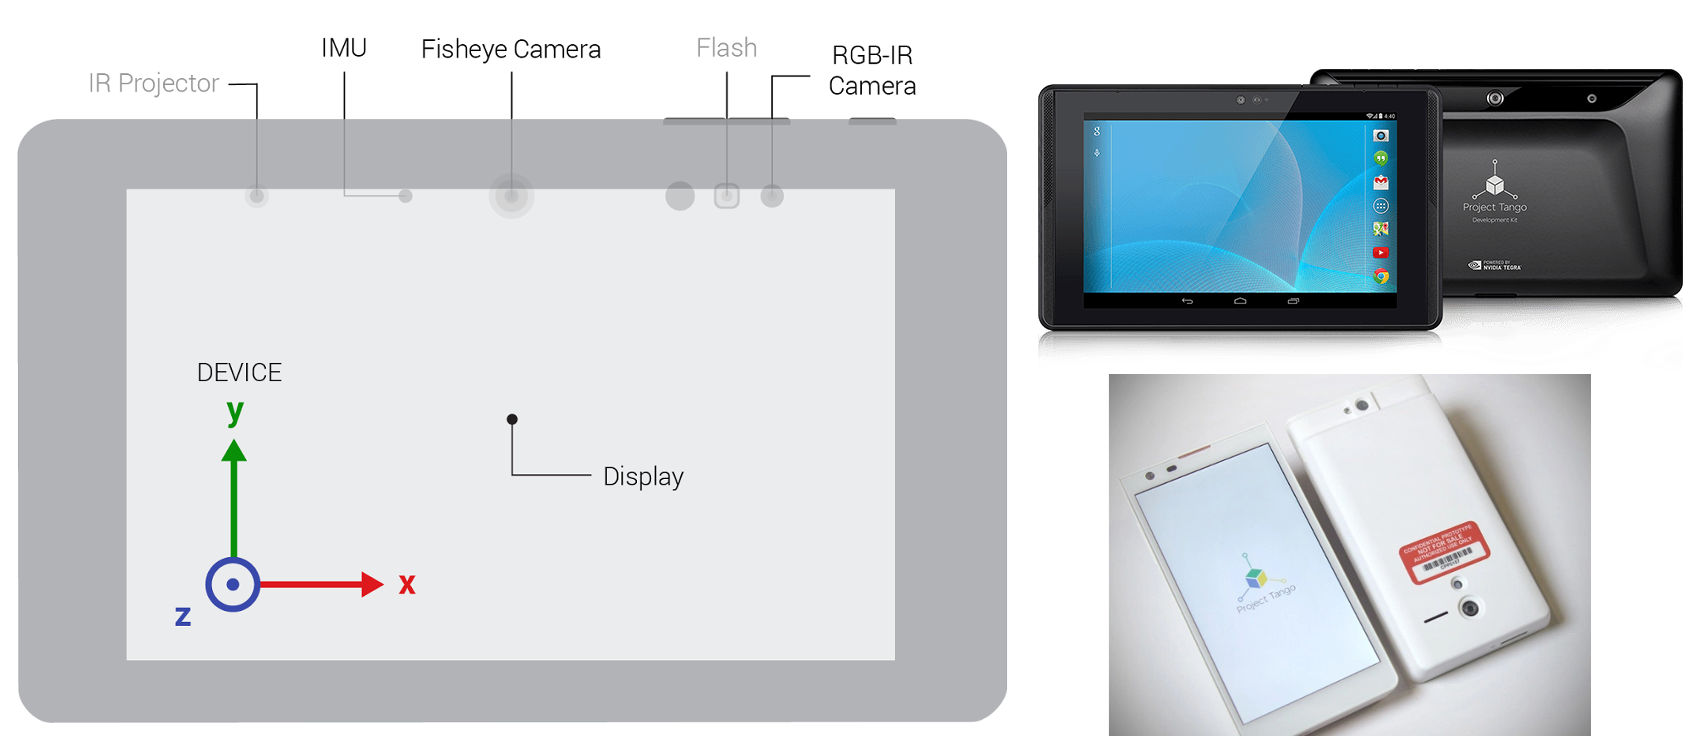
\includegraphics[width=1.0\textwidth]{content/images/theory/tango-device.png} 
  \caption{Links: schematischer Aufbau der Google Project Tango Hardware. Rechts: Das aktuelle Entwickler Gerät im Tablet Faktor (oben) und das alte Entwickler Gerät im Smartphone Faktor (unten). Übernommen von \citet{GoogleDevelopers:online}}
  \label{fig:tango-device}
\end{figure}

\subsection{Konzepte und Schnittstellen}

Generell betrachtet ist das Project Tango eine Plattform, die Computer Vision nutzt, um dem Gerät die Möglichkeit bietet seine relative Positionierung in der umgebenen Szene live zu bestimmen. Auf den Geräten kommt Googles Android zum Einsatz, weshalb zu beachten ist, dass es sich bei der Platform nur Bedingt um eine Echtzeit Umgebung handelt. Das liegt daran, dass der Linux Kernel keine Garantien für die zeitlich präzise Ausführung von Instruktionen  auf Grund von Scheduling geben kann. Google weist daher darauf hin, dass das System als \enquote{soft-realtime} betrachtet werden sollte. Daher sollten Messergebnisse verschiedener Sensoren unter Berücksichtigung ihrer Aufnahme Zeitstempel verwendet werden. \citep{GoogleDevelopersConcepts:online}

\subsubsection{Motion Tracking}

Um die relative Bewegung vom Start des Project Tango Systems bestimmen zu können nutzt es \enquote{visual-inertial odometry}. \citep{GoogleDevelopersConcepts:online}
Dabei handelt es sich um eine erweiterte Variante von Visual Odometry. 
Das von \citet{nister2004visual} veröffentlichte Verfahren Visual Odometry ist in der Lage aus einfachen Video Inhalten in Echtzeit die Bewegung der Kamera zu bestimmen. 
Hierzu werden zunächst übergreifende Features, zum Beispiel Punkte aus der \citet{harris1988combined} Kantenerkennung, über mehrere Bilder des Videos bestimmt, woraus mit Hilfe des 5-point Algorthmus und durch Answendung von RANSAC eine bestmögliche Approximation der Kamera Transformation bestimmt wird. \citep{nister2004visual}

Project Tango lässt an dieser Stelle die internen Sensoren zur Rotation, Orientierung und Bewegung mit in die Bestimmung der Kamera Transformation einfließen um so ein akurateres Ergebnis erziehlen zu können. Über eine längere Messzeit oder eine größere Entfernung vom Ursprung kann es jedoch zu kleinen Abweichungen kommen. Außerdem existiert zum aktullen Zeitpunkt noch ein \enquote{drift} Problem, was zu großen Messfehlern führen kann. Es wird jedoch versucht diese Probleme mit dem Konzept \enquote{Area Learning} aus Kapitel\ref{subsec:area-learning} zu lösen. \citep{GoogleDevelopersConcepts:online}
Wie genau das Verfahren aussieht, welche Techniken zur Feature Detection oder Feature Matching genutzt wird und welche Features hierfür erkannt werden ist nicht bekannt. 

\subsubsection{Deph Perception}

\subsubsection{Area Learning}


\subsection{Einordnung zu Augmented Reality}

Um das Project Tango in den zuvor erwähnten technologischen Charakteristika einordnen zu können, wird zunächst einmal auf die technischen Details der Plattform eingegangen. 
